\chapter{Simulating a system at negative temperature}

\section{The Ising Model}
Brief introduction to the Ising Model

\section{Single system at negative temperature}

\section{Two systems into contact}
Two systems are prepared at temperature $T_1$ and $T_2$. The spin configurations are obtained after $10^4$ Monte Carlo cycles in the canonical ensemble. \\
After that, the two systems are put into contact forming a new system that can be threated as a microcanonical ensemble. The simulation of the latter was obtained with a 
demon Monte Carlo method with $10^6$ cycles.

\begin{figure}[h]
    \centering
    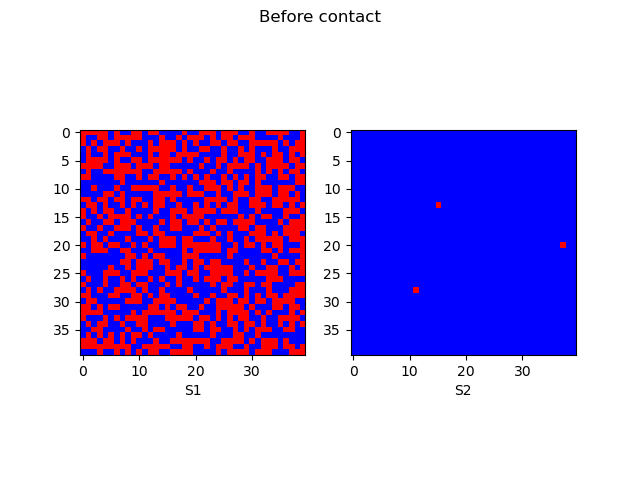
\includegraphics[scale=0.7]{./images/T1_T2_before.png}
    \caption{Before contact}{The red tiles indicate the \emph{up} state, while the blue tiles indicate the \emph{down} state. Before beeing put into contact
    the two systems are prepared respectively at temperature $k_B T_1 = -\infty \, (10^8)$ and $k_B T_2 = 0^+ \, (10^{-8})$}
    \label{fig:before}
\end{figure}

\begin{figure}[h]
    \centering
    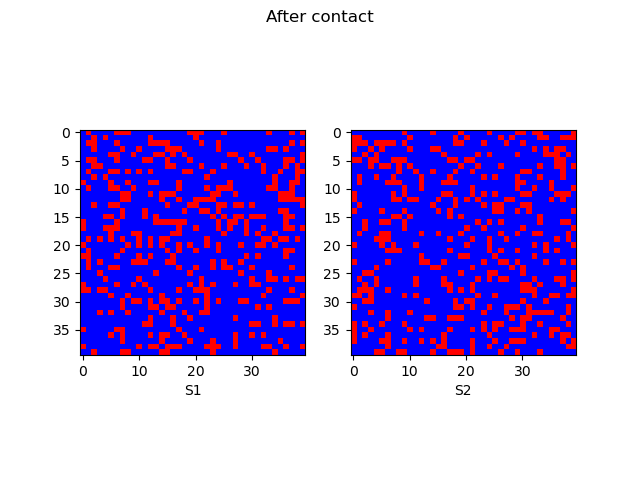
\includegraphics[scale=0.7]{./images/T1_T2_after.png}
    \caption{After contact}{The red tiles indicate the \emph{up} state, while the blue tiles indicate the \emph{down} state. The equilibrium temperature after putting the two systems into contact is in between the two values according to the hierarchy presented 
    at the end of chapter \ref{ch:temperature}. The system at negative temperature get cooled down changing some up states to down states, while the system at positive temperature
    gets heated changing some down states into up. The resuls is of course an approximately equal concentrarion of up/down in both systems.}
    \label{fig:after}
\end{figure}